% Chapter Template

\chapter{Microsoft Graph foundations} % Main chapter title

\label{Chapter2} % Change X to a consecutive number; for referencing this chapter elsewhere, use \ref{ChapterX}

%----------------------------------------------------------------------------------------
%	SECTION 1
%----------------------------------------------------------------------------------------

\section{Overview}

Microsoft Graph is a gateway to data and intelligence in Microsoft 365. It provides a unified programmability model that you can use to access data in Microsoft 365. Microsoft Graph can further be used to build apps for organizations and consumers that interact with millions of users \cite{MSGraphOverview} .

In Microsoft Graph there is a single endpoint that provides access to data in the Microsoft Cloud, including Microsoft Office. REST APIs can be used to access the endpoint and build applications that enable manipulating an Excel workbook for example. As part of Microsoft Graph, organisations can also manage user and device identity, access, compliance, and security, as well as protect against data leakage and loss \cite{MSGraphOverview}.

Inbound Connectors for Microsoft Graph carry data inside the Microsoft cloud and deliver it to Microsoft Graph services and applications, such as Microsoft Search. Apart from that, many common data sources outside the Microsoft universe are available via connectors, such as Google Drive, Jira and Salesforce \cite{MSGraphOverview}.

For Azure development tools, you can use the cached data as a source of data for developing intelligent applications.
Microsoft Graph API, connectors, and Data Connect together form the basis of the 365 platform. As a result of your ability to access Microsoft Graph data and other datasets, you can get insights and create your own applications \cite{MSGraphOverview}.


With regards to the objective of this VT, Microsoft Graph can be used by the web-based application to read and modify Excel workbooks stored on OneDrive for Business, a SharePoint site, or a group drive. A workbook can be accessed through the Drive API by specifying its location in the URL. The format of the URL looks as follows:
\\

https://graph.microsoft.com/v1.0/me/drive/items/{id}/workbook/  
\\[0.5cm]
Each file in OneDrive gets an id assigned which needs to be considered in the path. By using the standard REST APIs, a user can access a set of Excel objects such as a range of cells and perform CRUD operations (create, read, update, and delete) on the workbook. 


%----------------------------------------------------------------------------------------
%	SECTION 2
%----------------------------------------------------------------------------------------

\section{Authentication and authorization}

Your users and customers can utilize the Microsoft Identity Platform to sign into your applications using their Microsoft identities or social accounts, and give them access to Microsoft Graph. In the process OAuth 2.0 and OpenID Connect (OIDC) flows are used for Authentication and authorization respectively \cite{MSIDP}. In OAuth 2.0 the following roles as shown in \ref{fig:roles for Microsoft Graph} are defined in the context of Microsoft Graph \cite{MSOAuthOIDr}:

\begin{figure}[h!]
  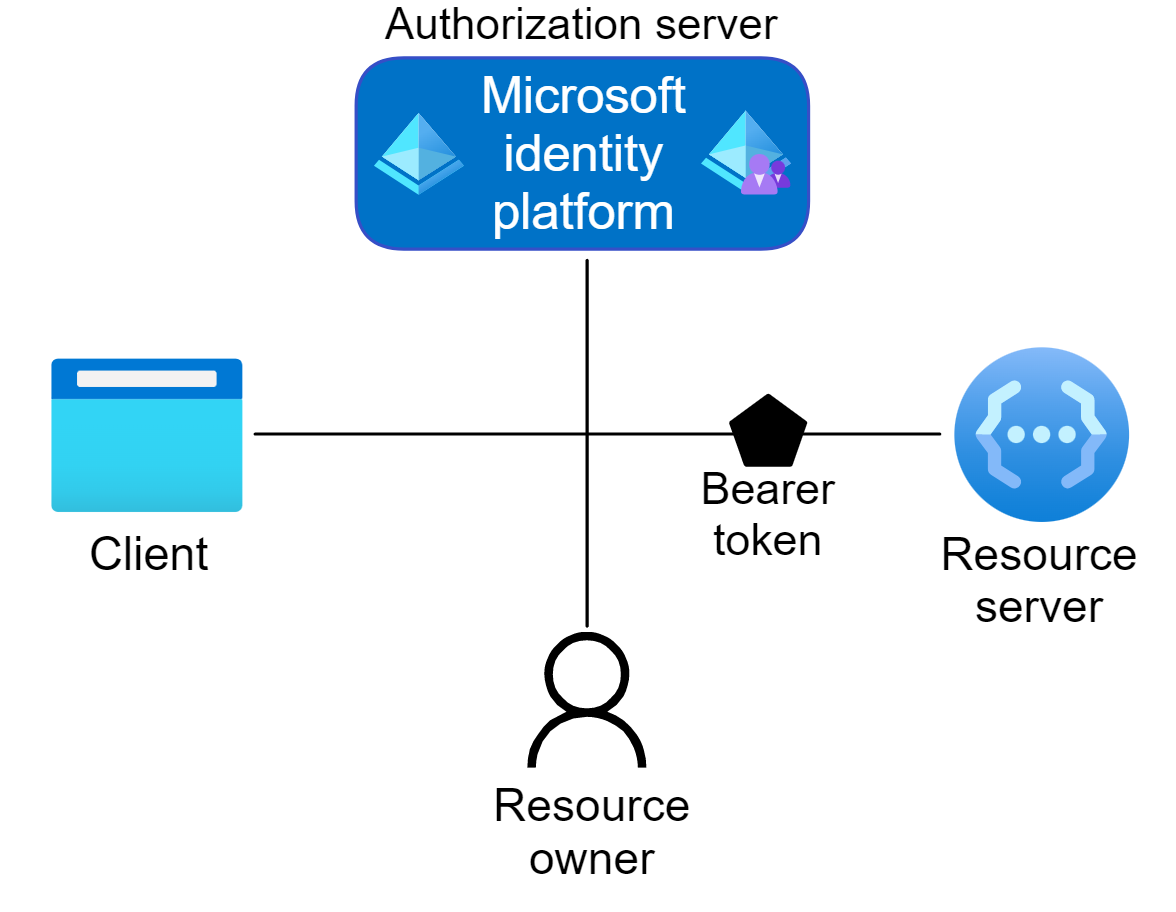
\includegraphics[scale=0.9]{Figures/OAuth roles.png}
  \caption{roles for Microsoft Graph}
  \label{OAuth 2.0 roles for Microsoft Graph}
\end{figure}

\begin{itemize}
 \item Authorisation server: The Microsoft Identity Platform serves as the authorization server. In addition, it performs the function of an identity provider (IdP) since it maintains Microsoft accounts and oversees the trust relationship between parties during the authentication process. Authorization servers create security tokens after a user logs in (authenticates) to grant, deny or revoke access to resources (authorization) \cite{MSOAuthOIDr}.
 \item Client: The client in this context is your application you created and registered on the Microsoft Identity platform. It requests access to protected resources as soon as it being used. Depending on the client, it can be a server-based web application, a user-facing one-page web application, or a web API that interacts with another web API \cite{MSOAuthOIDr}. 
 \item Ressource Owner: An application user is usually the resource owner in an authentication flow. Your application wants to access the users data on the ressource owners behalf. The owner of the resource can grant or deny your application (the client) access to the resources it owns \cite{MSOAuthOIDr}. 
 \item Resource server: The resource server hosts or provides access to data owned by a resource owner. A data store is usually preceded by a web API serving as a resource server. Access to resources is controlled by the resource server using information in owner tokens issued by the authentication server \cite{MSOAuthOIDr}. 
\end{itemize}

A flow of authentication uses bearer tokens to guarantee identification (authentication) and to grant or deny access to protected resources (authorization). JSON Web Tokens (JWT) are formatted for bearer tokens in Microsoft Identity Platform. A bearer token may be one of three types used by the Microsoft Identity Platform as a security token:

\begin{itemize}
 \item Access tokens: The authorisation server issues access tokens to the client application. The client then passes these tokens on to the resource server. Access tokens are further sent from Authorisation servers to the client to declare which resources and APIs your app has access to \cite{MSOAuthOIDr}. It includes information (claims) that is verified using web APIs protected by the platform, such as Microsoft Graph, to determine whether the user has the necessary permissions to execute the request. An HTTP request with an Authorization header must include the access token attached as a Bearer token \cite{MSAA}.
 \item ID tokens: The client application receives ID tokens from the authorisation server. A client uses an ID token to enroll users and to gain basic information about them.
 \item Refresh tokens: Clients use refresh tokens to request new access and ID tokens from the authorization server.
\end{itemize}


Obtaining security tokens from Microsoft Identity Platform is the crucial step in accessing Microsoft Graph. Security tokens for Microsoft Graph can only be acquired if your application is registered with the Microsoft Identity Platform and authorised to access them by either a user or administrator. Through registration, your application (client) can trust the security tokens issued by the Microsoft Identity Platform \cite{MSAA}.

It is mandatory for your application to be registered in the Azure Portal as through registration, you connect your application to Microsoft Identity Platform and define the information it uses for security token retrieval, including:

\begin{itemize}
 \item An application ID that is unique to your application.
 \item Redirect URI/URL: One or more endpoints from which the Microsoft Identity Platform responds to your application.
 \item Client secret: Your application will use your client secret to authenticate to the Microsoft Identity Platform using a password or public/private key pair \cite{MSAA}.
\end{itemize}

When it comes to choosing Microsoft Graph permissions for your application, it is up to you as a developer to select these permissions in the Azure Portal. An administrator, or depending on the scenario a user, is given the option to accept these permissions when they log into your application. Users can grant your application access to the requested resources and APIs if they agree. An administrator can preapprove permissions for applications that access resources without requiring a user to log in before. There are two types of permissions in Microsoft Graph which are delegated and application permissions \cite{MSAA}.

Applications with logged-in users use delegates permissions. Users or administrators must approve the application's permissions in order for Microsoft Graph to work with these applications. The application can then act as the logged-in user. Non-administrative users can approve some delegated permissions, but some higher-privileged permissions require administrative approval \cite{MSAA}.

There can also be applications running without an logged-in user. These applications utilize application permissions. Examples include background services and daemons. Only administrators can approve application permissions \cite{MSAA}.

For managing token interactions with the Microsoft Identity Platform, developers typically use authentication libraries. As a developer, you can focus on the functionality of your application while authentication libraries handle many protocol details such as cookie processing, token caching, and maintaining secure connections. Several Microsoft open source client libraries are also available \cite{MSAA}.

In order to use the Microsoft identity platform endpoint there are Microsoft Authentication Library (MSAL) client libraries for .NET. As part of their implementation of the Microsoft Authentication Library (MSAL), authentication providers implement the code required to acquire a token, handle errors such as incremental consent, expired passwords, and conditional access, and set the HTTP request authorisation header. Listed below are the providers that correspond to the different types of applications. According to the table each scenario and application type match a different authentication provider \cite{MSAuthPr}.

\begin{figure}[h!]
  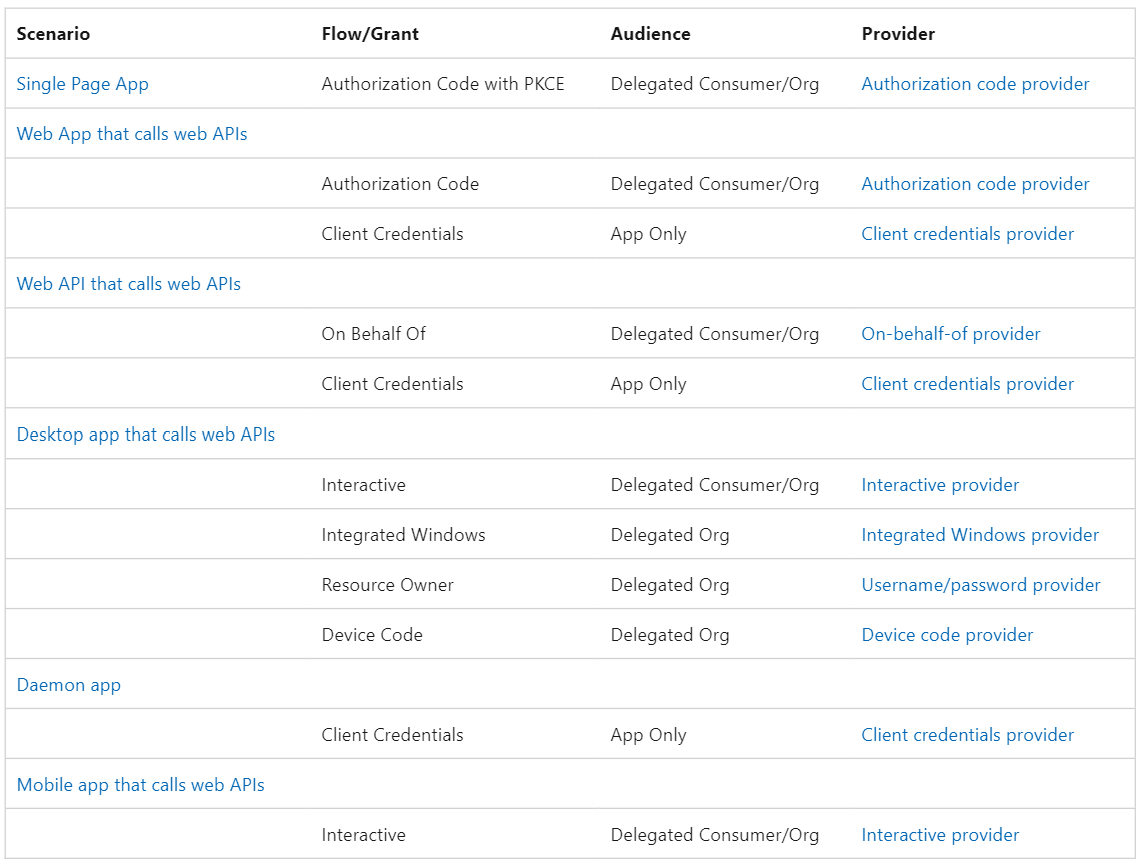
\includegraphics[scale=0.95]{Figures/Authentication providers.png}
  \caption{Authentication providers according to scenario}
  \label{fig:Authentication providers according to scenario}
\end{figure}

Depending on the selected authentication flow and the according provider, the user will be asked to login in his Microsoft account so that the web app can obtain an access token or the application is enabled to run without user interaction. The former is for example the case for the authorization code provider, while the latter is the case for the client credentials provider \cite{MSAuthPr}.









